En esta sección el objetivo será comparar todos los algoritmos heurísticos diseñados e implementados en este trabajo, contrastando tanto el tiempo de ejecución como la calidad de las soluciones obtenidas.


En una primera instancia, estudiamos el comportamiento de las heurísticas al resolver instancias sobre grafos generados al azar. Luego, pasamos a observar cómo se comportan ante la familia de grafos \emph{3-caminos}, y ante la familia \emph{3-caminos con puentes}.

Para los siguientes gráficos, vamos a utilizar grafos ralos y luego densos. La cantidad de aristas en el grafo random va a ser $m$, donde $m$ = $m^*$ $*$ $\#(E(K_n))$. Por otro lado, definimos la cota como $K$, donde $K = K^* * \frac{n}{2} * \frac{max_{w_1}}{2}$. 

%TODO EXPLICAR ESTOS NUMEROS MAGICOS? ^

Para cada $n$, calculamos 10 instancias diferentes usando las tres heurísticas. Para cada instancia y por cada heurística, nos quedamos con el siguiente valor:

\begin{center}
$\frac{w_2}{w_2 promedio}$
\end{center}

donde $w_2 promedio$ es el valor promedio de los $w_2$ resultantes de correr cada heurística para dicha instancia.

Ahora, como para cada $n$ tenemos 10 instancias, calculamos (para cada $n$) el promedio de los valores que obtuvimos en el paso anterior.

Esto generaba que los gráficos tengan valores cercanos a uno, por lo que restamos uno al final.

\begin{figure}[H]
    \begin{minipage}{0.5\linewidth}
      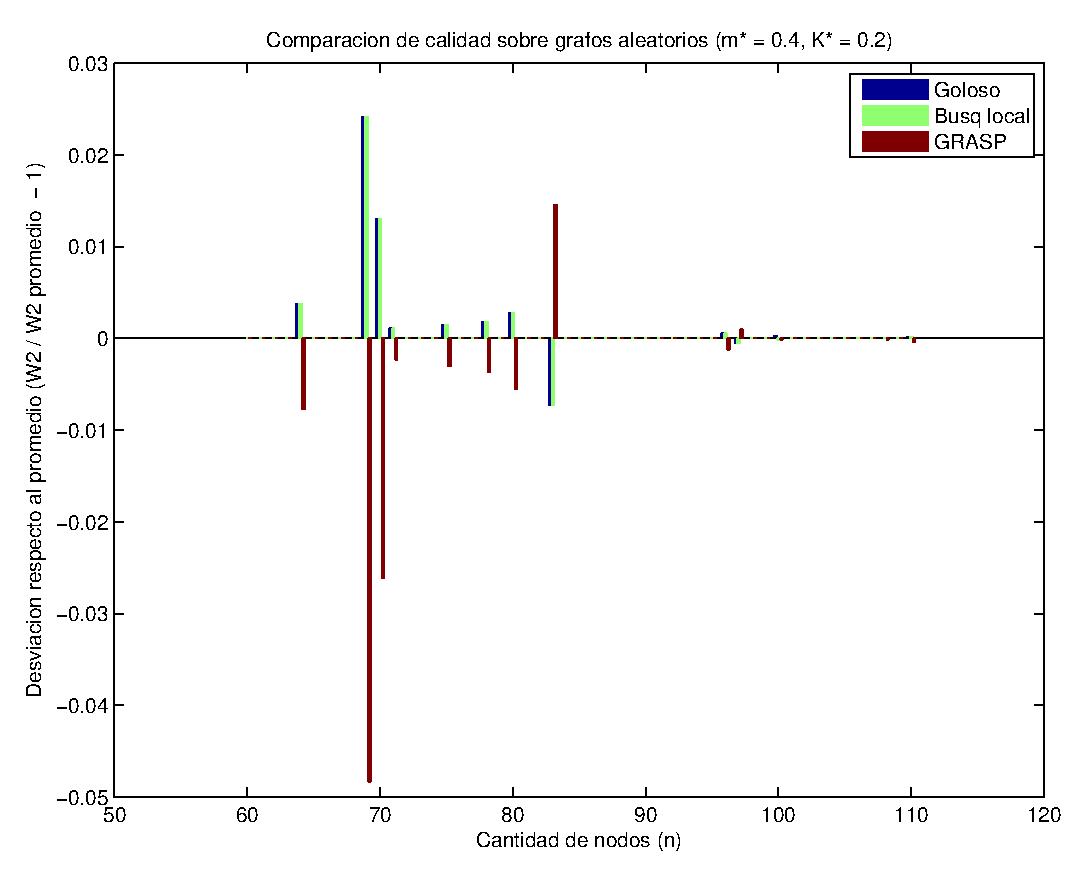
\includegraphics[width=\linewidth]{graficos/todos_calidad_m04_K02.eps}
      \caption{Calidad grafos ralos aleatorios, cota ajustada}\label{fig:ralos-ajustada}
    \end{minipage}
    \hfill
    \begin{minipage}{0.5\linewidth}
      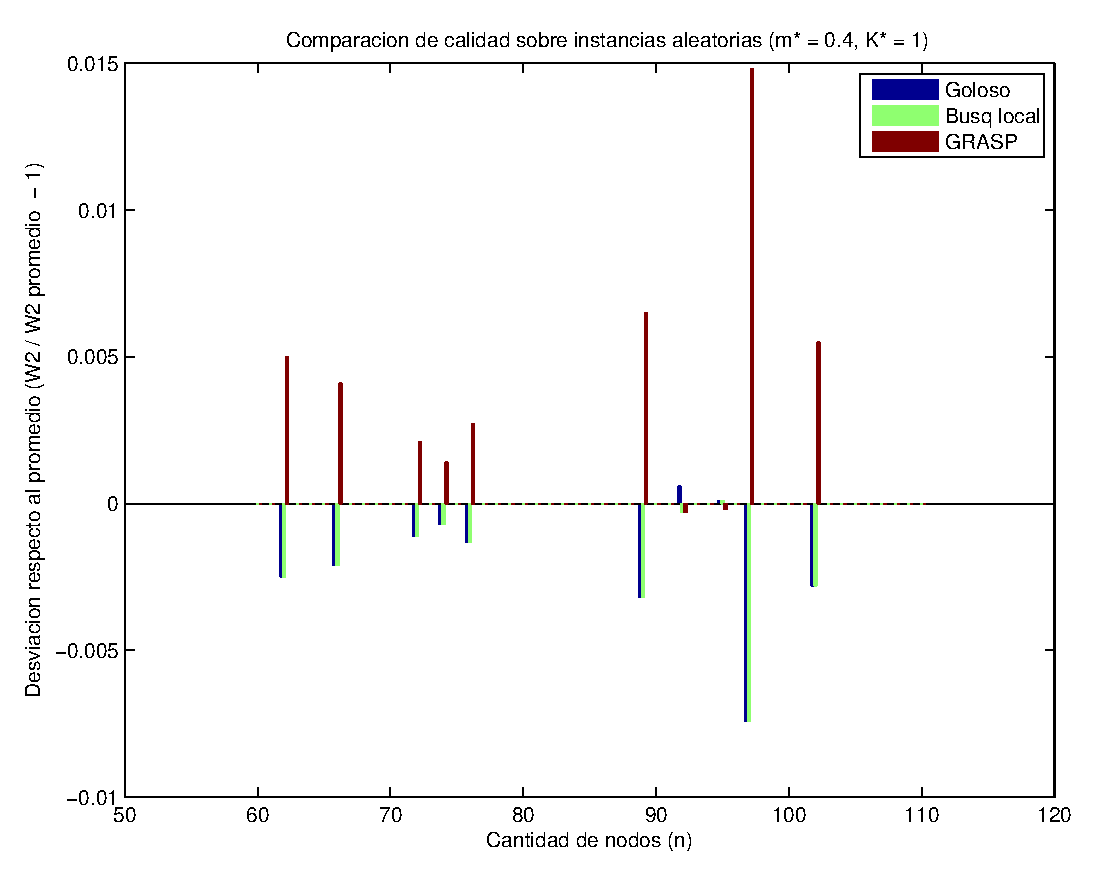
\includegraphics[width=\linewidth]{graficos/todos_calidad_m04_K1.eps}
      \caption{Ídem, cota libre}\label{fig:ralos-libre}
    \end{minipage}    
\end{figure}

Podemos observar en las Figuras \ref{fig:ralos-ajustada} y \ref{fig:ralos-libre} que en la mayoría de los casos, las tres heurísticas producen resultados similares.

En la Figura \ref{fig:ralos-ajustada} podemos observar que el algoritmo GRASP logra mejorar respecto del algoritmo goloso y del algoritmo de búsqueda local. Por otro lado, en la Figura \ref{fig:ralos-libre} GRASP es peor que las otras dos heurísticas en la mayoría de casos donde no son iguales. De estos gráficos podemos concluir que el algoritmo de GRASP se comporta mejor con cota ajustada contra utilizar una cota libre.

El algoritmo de búsqueda local siempre da soluciones que son mejores o iguales a las que da el algoritmo goloso (para un mismo $n$), ya que la proporción es siempre menor o igual a uno. Esto es lógico ya que nuestro algoritmo de búsqueda local toma como solución inicial la que da el goloso e intenta mejorarlas, lo cual no siempre logra, pero nunca empeora la solución inicial que se le da.


\begin{figure}[H]
    \begin{minipage}{0.5\linewidth}
      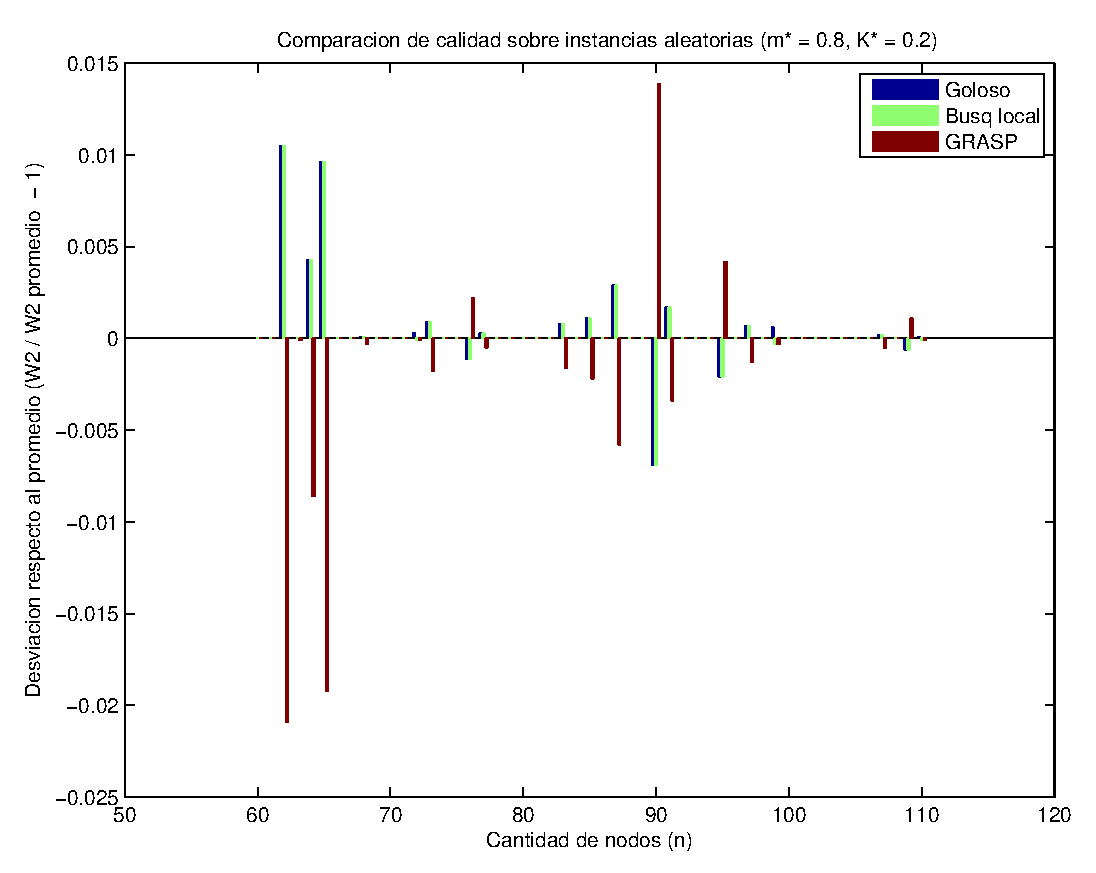
\includegraphics[width=\linewidth]{graficos/todos_calidad_m08_K02.eps}
      \caption{Calidad grafos densos aleatorios, cota ajustada}\label{fig:densos-ajustada}
    \end{minipage}
    \hfill
    \begin{minipage}{0.5\linewidth}
      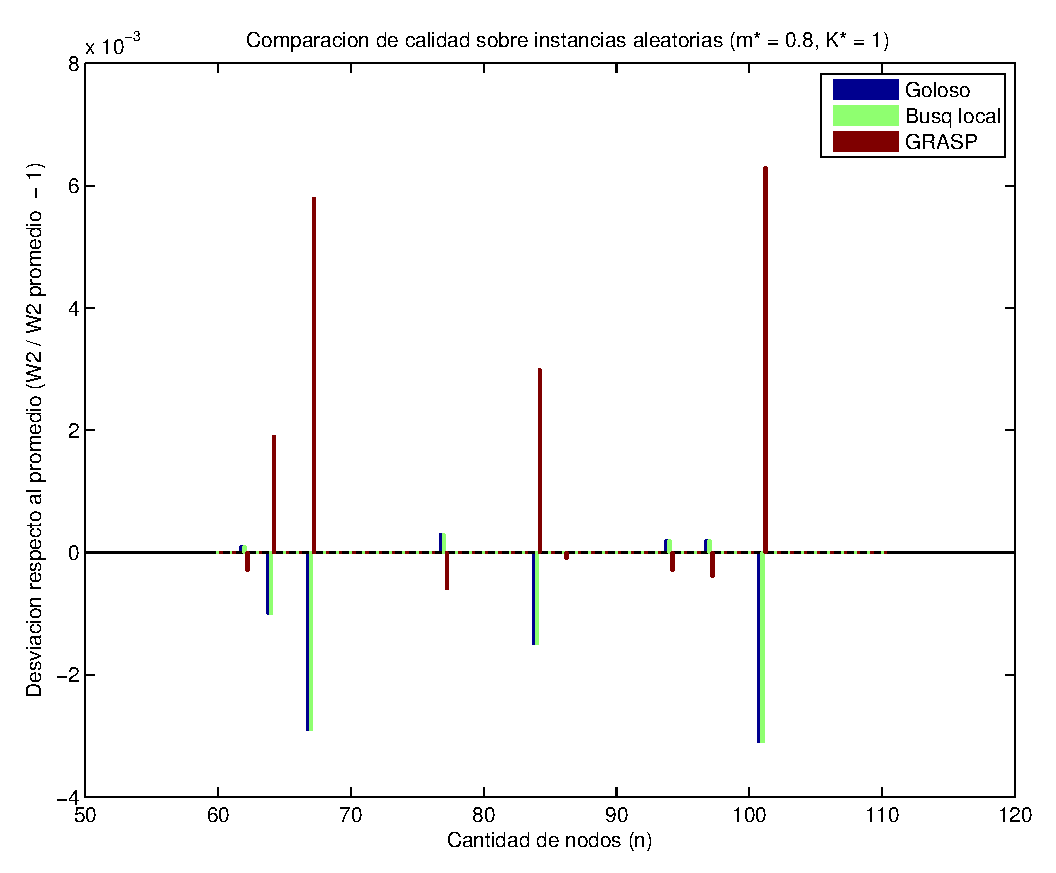
\includegraphics[width=\linewidth]{graficos/todos_calidad_m08_K1.eps}
      \caption{Ídem, cota libre}\label{fig:densos-libre}
    \end{minipage}    
\end{figure}

En estos dos gráficos, podemos observar resultados similares a las Figuras \ref{fig:ralos-ajustada} y \ref{fig:ralos-libre}. Una vez más, las tres heurísticas producen resultados similares, en en la mayoría de los casos.

GRASP logra mejorar en algunos casos respecto del algoritmo goloso y del algoritmo de búsqueda local cuando la cota es ajustada, pero es peor en general donde la cota es libre.

También, los algoritmos goloso y búsqueda local tienen resultados similares para los distintos $n$.

Por todo esto, creemos que dado un grafo cualuiera, nuestro algoritmo de GRASP se comporta mejor cuando la cota es ajustada, y la cantidad de aristas no es un factor crucial en el resultado de dicho algoritmo.

Además, podemos ver que las soluciones que da el algoritmo GRASP son a veces mejores que las del algoritmo de búsqueda local pero a veces son peores. Esto es debido a que el algoritmo de GRASP hace búsqueda local sobre la solución inicial que le da nuestro algoritmo goloso aleatorio en cada iteración. Por lo tanto, GRASP hace búsqueda local a partir de soluciones iniciales distintas a la del algoritmo de búsqueda local que toma como solución inicial la dada por nuestro algoritmo goloso que no es aleatorio. Entonces, tiene sentido que GRASP llegue a soluciones distintas al algoritmo de búsqueda local, las cuales a veces son mejores y a veces son peores.

Otro punto que vale la pena destacar es que no hay una gran variación entre las soluciones ($ \pm 10\%$)


%TODO Este ultimo grafico lo dejamos?

% Para continuar incluimos un gráfico que compara las soluciones de nuestro algoritmo GRASP y nuestro algoritmo de búsqueda local en proporción con nuestro algoritmo goloso.
% 
% \begin{figure}[H]
%   \begin{center}
%     \begin{minipage}{0.5\linewidth}
%     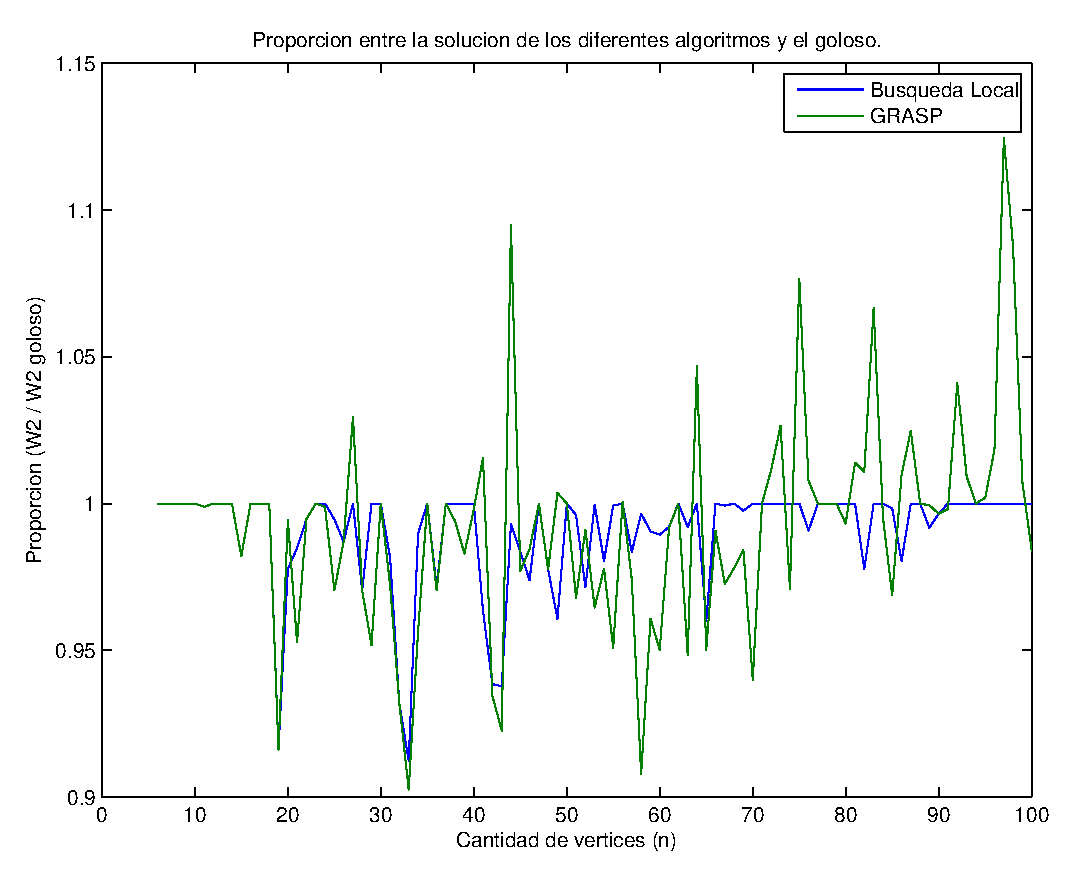
\includegraphics[width=\linewidth]{graficos/todos_calidad.eps}
%     \caption{Soluciones en proporción con goloso}\label{fig:proporcion-goloso}
%     \end{minipage}
%   \end{center}
% \end{figure}


Ahora vamos a observar como se comportan nuestros algoritmos ante la familia de grafos \emph{3-caminos} y otro ante la familia \emph{3-caminos con puentes}. Usamos $i$ = $n$ en ambas familias. Ver secciones \ref{subsub:algoritmos-heuristicos-goloso-calidad.tex} y \ref{subsub:algoritmos-heuristicos-busqueda-calidad.tex} para entender las familias.

Cabe aclarar que, para ambas familias, dado un $n$ existe una sola representación de las mismas. Por esto, para cada familia, graficamos una única instancia y no múltiples.

\begin{figure}[H]
    \begin{minipage}{0.5\linewidth}
      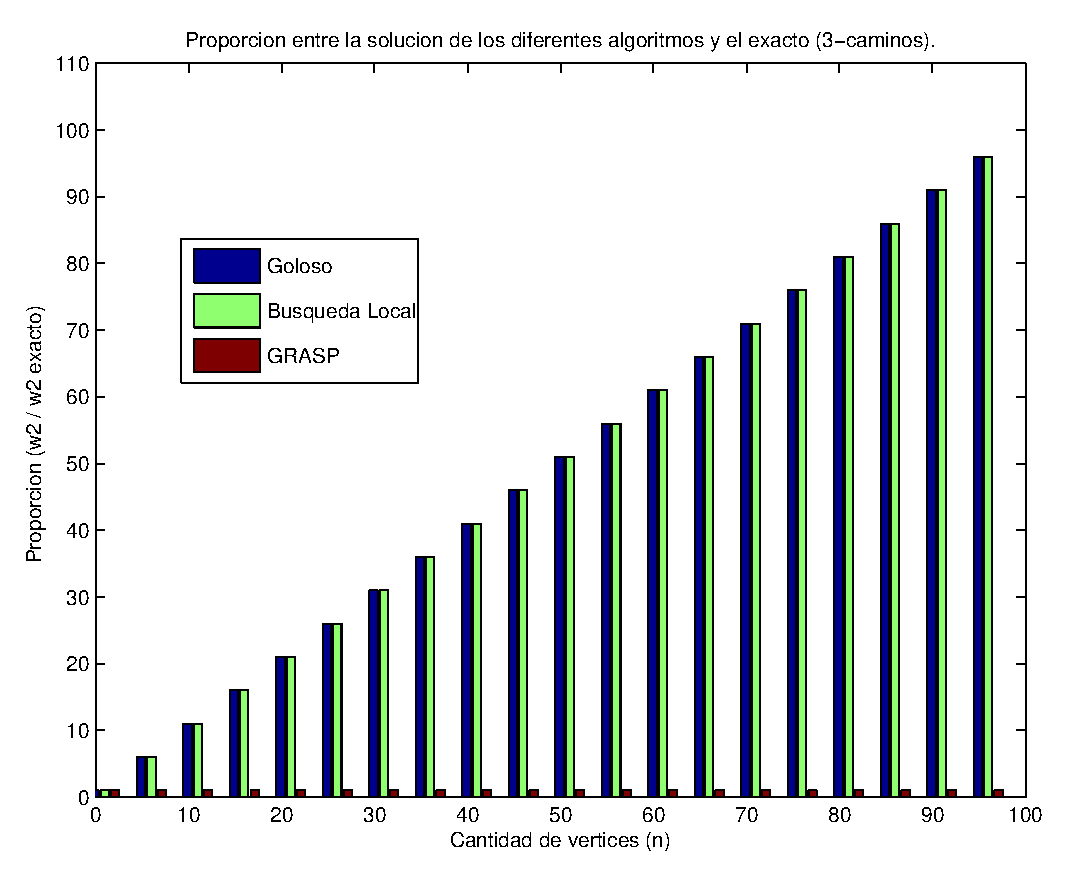
\includegraphics[width=\linewidth]{graficos/todos_proporcion_3caminos.eps}
      \caption{Comportamiento ante familia \emph{3-caminos}}\label{fig:comportamiento-familia-rompe}
    \end{minipage}
    \hfill
    \begin{minipage}{0.5\linewidth}
      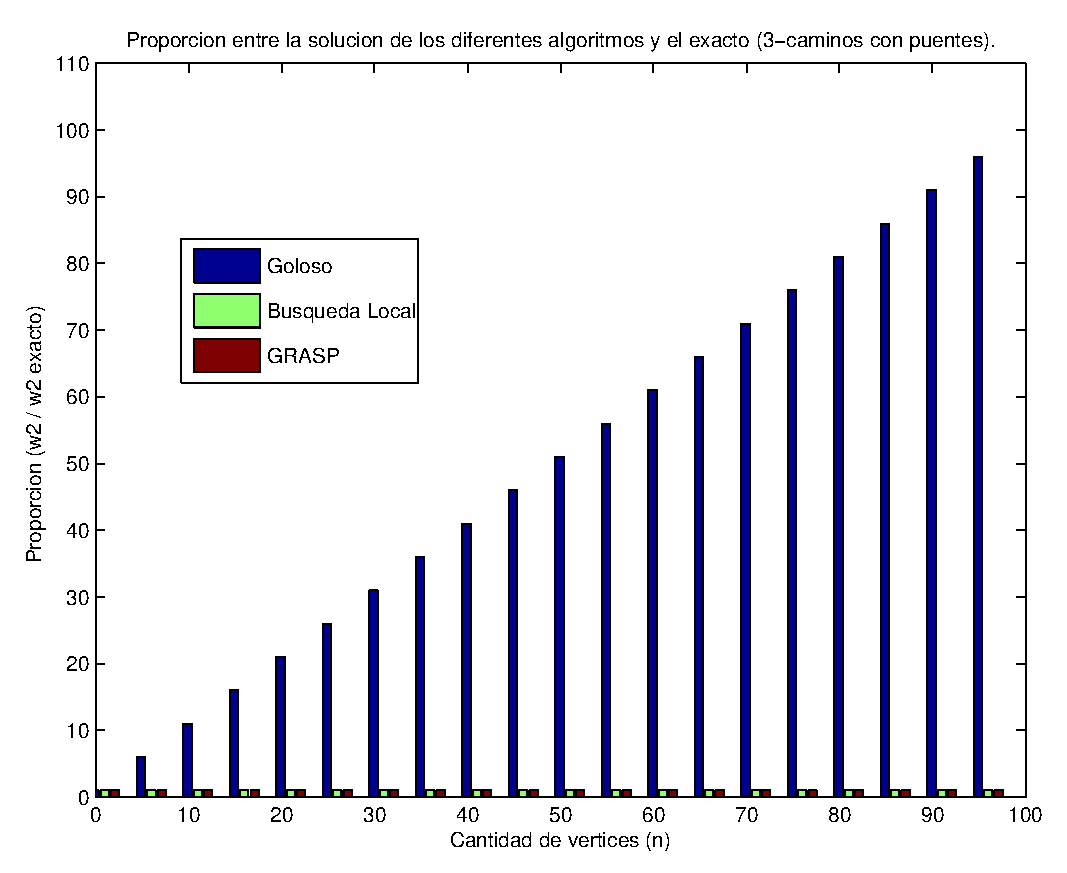
\includegraphics[width=\linewidth]{graficos/todos_proporcion_puentes.eps}
      \caption{Ídem familia \emph{3-caminos con puentes}}\label{fig:comportamiento-familia-puente}
    \end{minipage}    
\end{figure}

En los dos gráficos anteriores mostramos el comportamiento de los siguientes algoritmos para dos familias de grafos. Los algoritmos medidos son los siguientes:

\begin{itemize}
 \item Algoritmo Goloso implementado en el trabajo.
 \item Algoritmo de búsqueda local, que utiliza nuestro algoritmo goloso.
 \item Algoritmo GRASP que utiliza nuestro algoritmo goloso aleatorio y nuestro algoritmo de búsqueda local.
\end{itemize}

Vale aclarar que los parámetros utilizados en cada algoritmo son los mejores valores de configuración encontrados. Por otro lado, todas las soluciones se muestran en proporción a las del algoritmo exacto.

En el gráfico de la Figura \ref{fig:comportamiento-familia-rompe} podemos ver que para los grafos de la familia \emph{3-caminos} nuestro algoritmo goloso devuelve soluciones de mala calidad, al igual que nuestro algoritmo de búsqueda local. Sin embargo, nuestro algoritmo GRASP logra mejorar las soluciones de dichos algoritmos. Más aún, no solo las mejora sino que devuelve la solución óptima. También podemos volver a ver que nuestro algoritmo de búsqueda local no logra mejorar la solución inicial que le da el algoritmo goloso para esta familia de grafos cuando éstos superan una determinada cantidad de nodos (en secciones previas observamos que dicha cantidad es $7$).

A su vez, en el gráfico de la Figura \ref{fig:comportamiento-familia-puente} podemos observar que nuestro algoritmo goloso devuelve malas soluciones para la familia de grafos \emph{3-caminos con puentes}, pero que el algoritmo de búsqueda local las logra mejorar, devolviendo una solución óptima. También podemos ver que el algoritmo GRASP también se comporta de manera óptima para los algoritmos de dicha familia.

Finalmente, realizamos mediciones de tiempo para los algoritmos en estas dos familias.

\begin{figure}[H]
    \begin{minipage}{0.5\linewidth}
      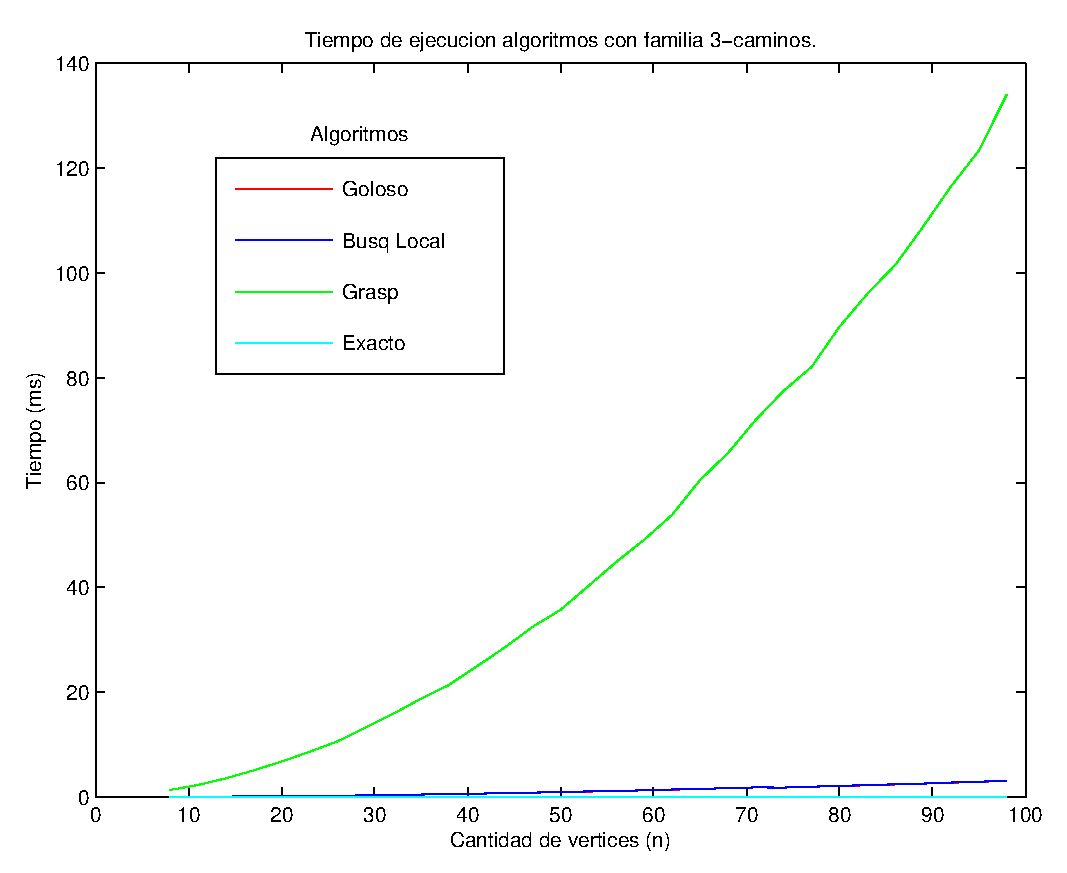
\includegraphics[width=\linewidth]{graficos/todos_tiempo_3caminos.eps}
      \caption{Tiempo de ejecución familia \emph{3-caminos}}\label{fig:3caminos-all}
    \end{minipage}
    \hfill
    \begin{minipage}{0.5\linewidth}
      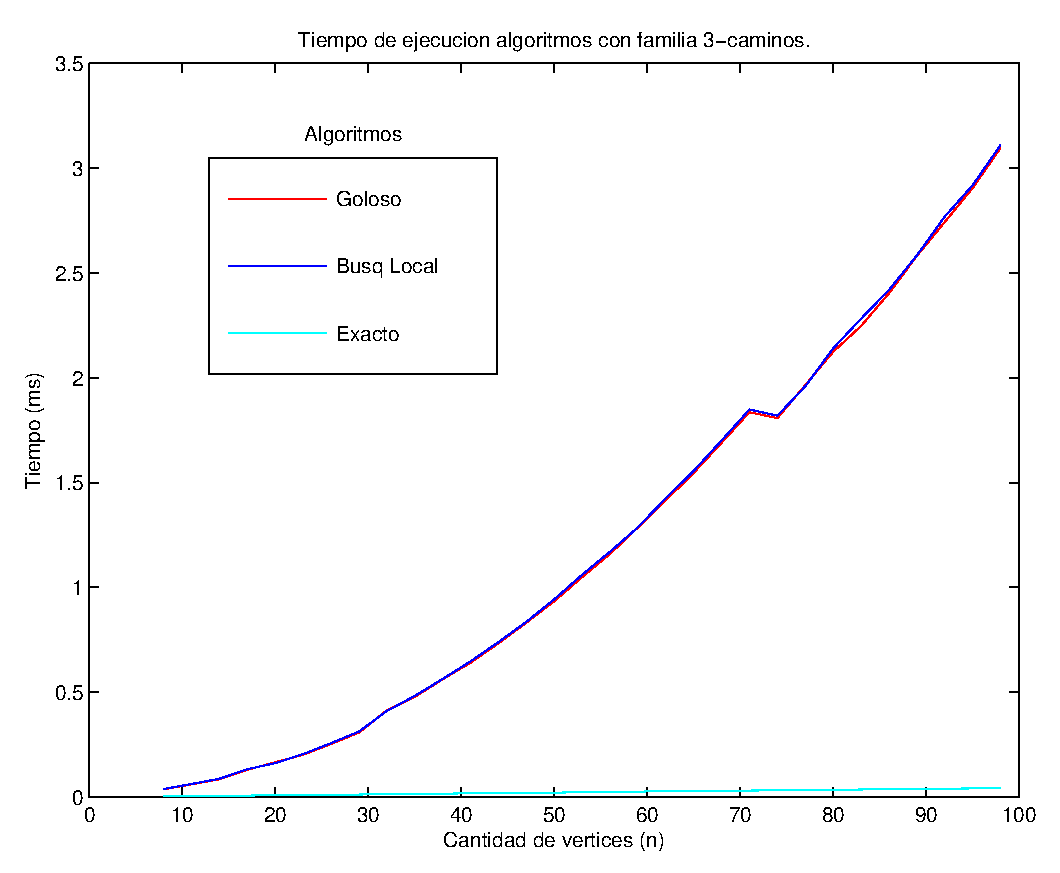
\includegraphics[width=\linewidth]{graficos/todos_tiempo_3caminos_sinG.eps}
      \caption{Ídem, sin GRASP}\label{fig:3caminos-sinG}
    \end{minipage}    
\end{figure}

Como podemos observar en la Figura \ref{fig:3caminos-all}, GRASP tarda considerablemente más tiempo que los otros algoritmos. Por esta razón, realizamos otro gráfico (Figura \ref{fig:3caminos-sinG}) removiendo el tiempo de ejecución de GRASP. Notamos que la búsqueda local y el algoritmo goloso tardan una cantidad de tiempo parecida, mientras que sorprendentemente el algoritmo exacto es mucho mejor. Creemos que esto se debe a que en esta familia de grafos, sólo existen tres caminos del nodo inicial al nodo final. Luego, el backtracking, va a recorrer dichos tres caminos, pasando una vez por cada nodo por lo que tiene una complejidad lineal.

Luego, vamos a analizar el tiempo de ejecución sobre la familia \emph{3-caminos con puentes}

\begin{figure}[H]
    \begin{minipage}{0.5\linewidth}
      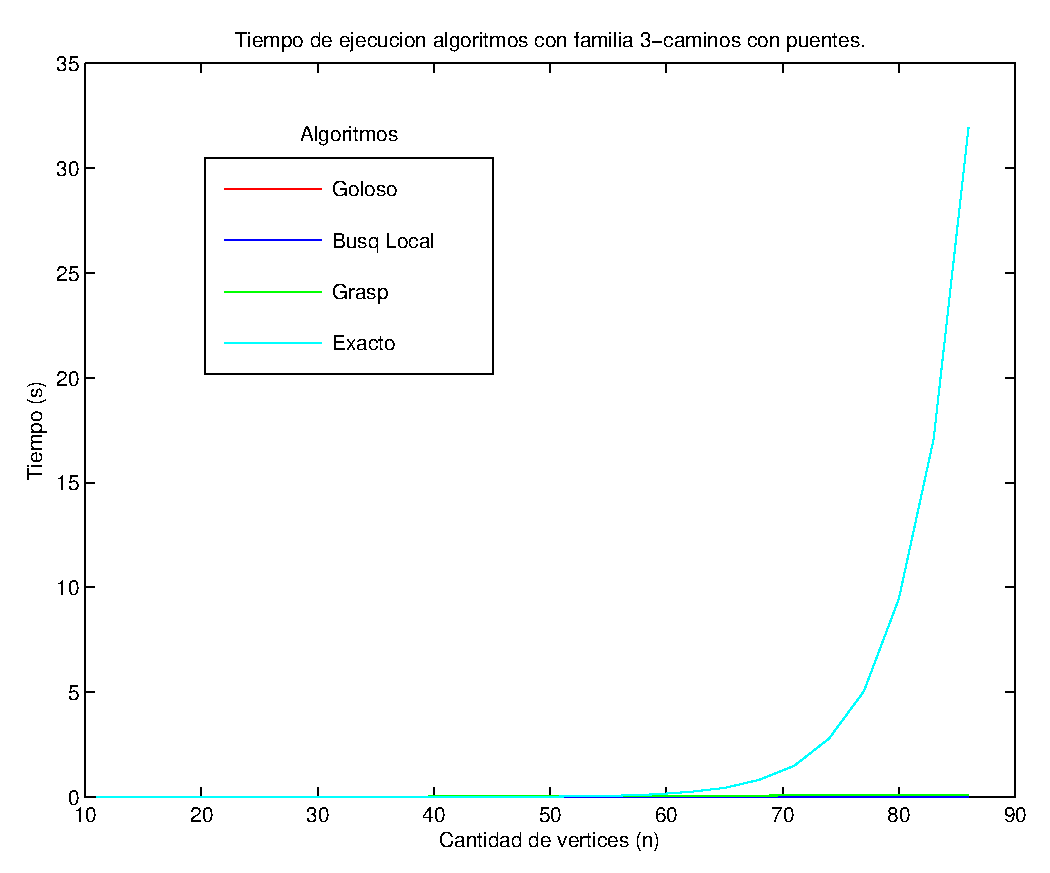
\includegraphics[width=\linewidth]{graficos/todos_tiempo_puentes.eps}
      \caption{Tiempo de ejecución familia \emph{3-caminos con puentes}}\label{fig:3caminospuente-all}
    \end{minipage}
    \hfill
    \begin{minipage}{0.5\linewidth}
      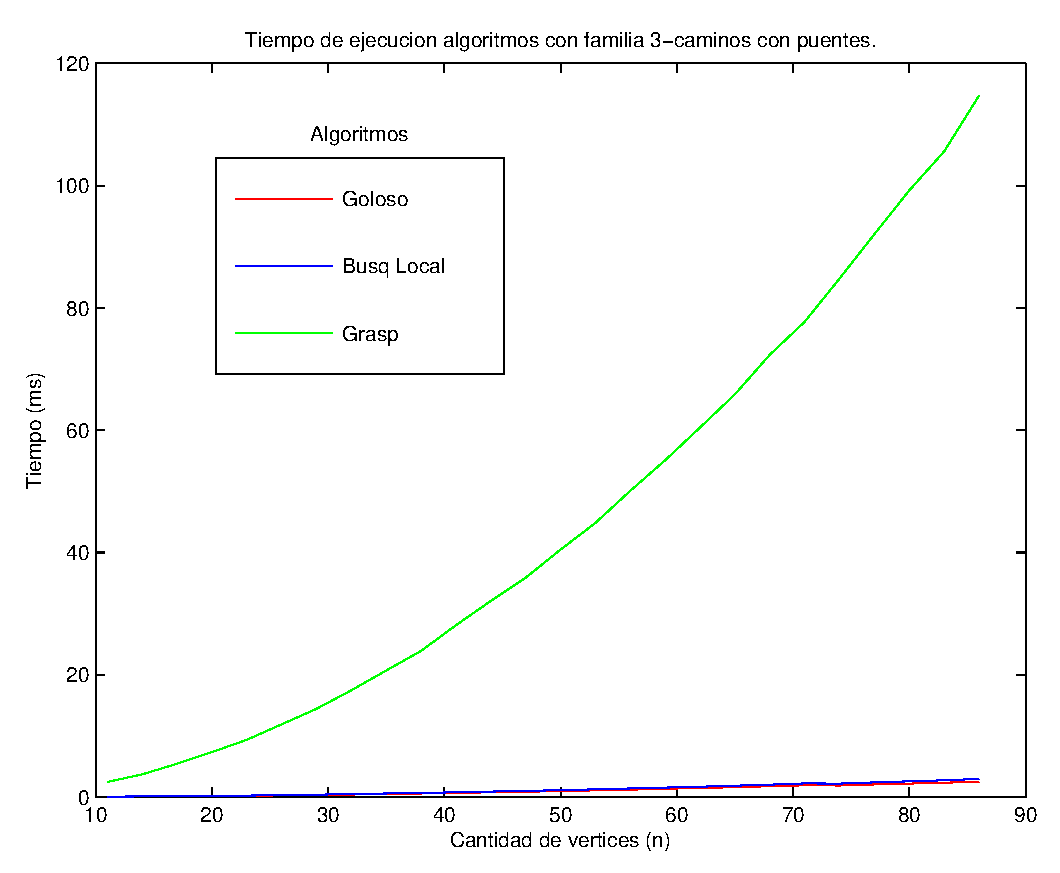
\includegraphics[width=\linewidth]{graficos/todos_tiempo_puentes_sinE.eps}
      \caption{Ídem, sin Exacto}\label{fig:3caminospuente-sinE}
    \end{minipage}    
\end{figure}

Podemos observar en la Figura \ref{fig:3caminospuente-all} que el algoritmo exacto tarda gran cantidad de tiempo con respecto a los demás algoritmos. Luego, decidimos hacer otro gráfico (Figura \ref{fig:3caminospuente-sinE}) que no contenga los resultados del algoritmo exacto para poder comparar los otros algoritmos.

Una vez más el tiempo de ejecución del algoritmo goloso y el algoritmo de búsqueda local son similares. Por otro lado, el algoritmo de GRASP tarda más que estos dos, pero no llega a tardar tanto como el algoritmo exacto.